\chapter{The Meta-layer}

\section{Data-flow schema}
In Apiis both ordinary SQL statements and PseudoSQL  \index{PseudoSQL} statements are allowed. From the standard SQL92 syntax only \'simple\' insert, update and delete can be used. These statements get parsed and  data are filled in  the internal part of record object where the access rights check against the user rights take place. After successfully passing the access rights check the statement is executed via the meta-user account in the database - just like the ordinary PseudoSQL statements.\linebreak
The ordinary Select statements can be very complicated and hard to parse therefore they follow different route - these statements are not parsed, but directly executed via user account  against the views in his own schema. These views are subset of the standard tables restricted with the user access rights, and have the same name as the original table. There the only item in the database that user has access to.
\linebreak The PseudoSQl statements get parsed, loaded in the external part of record object and then encoded, checked against access rights and executed via the meta-user account.
The flow is shown on \ref{fig:meta1} 
\begin{figure}
   \centering
   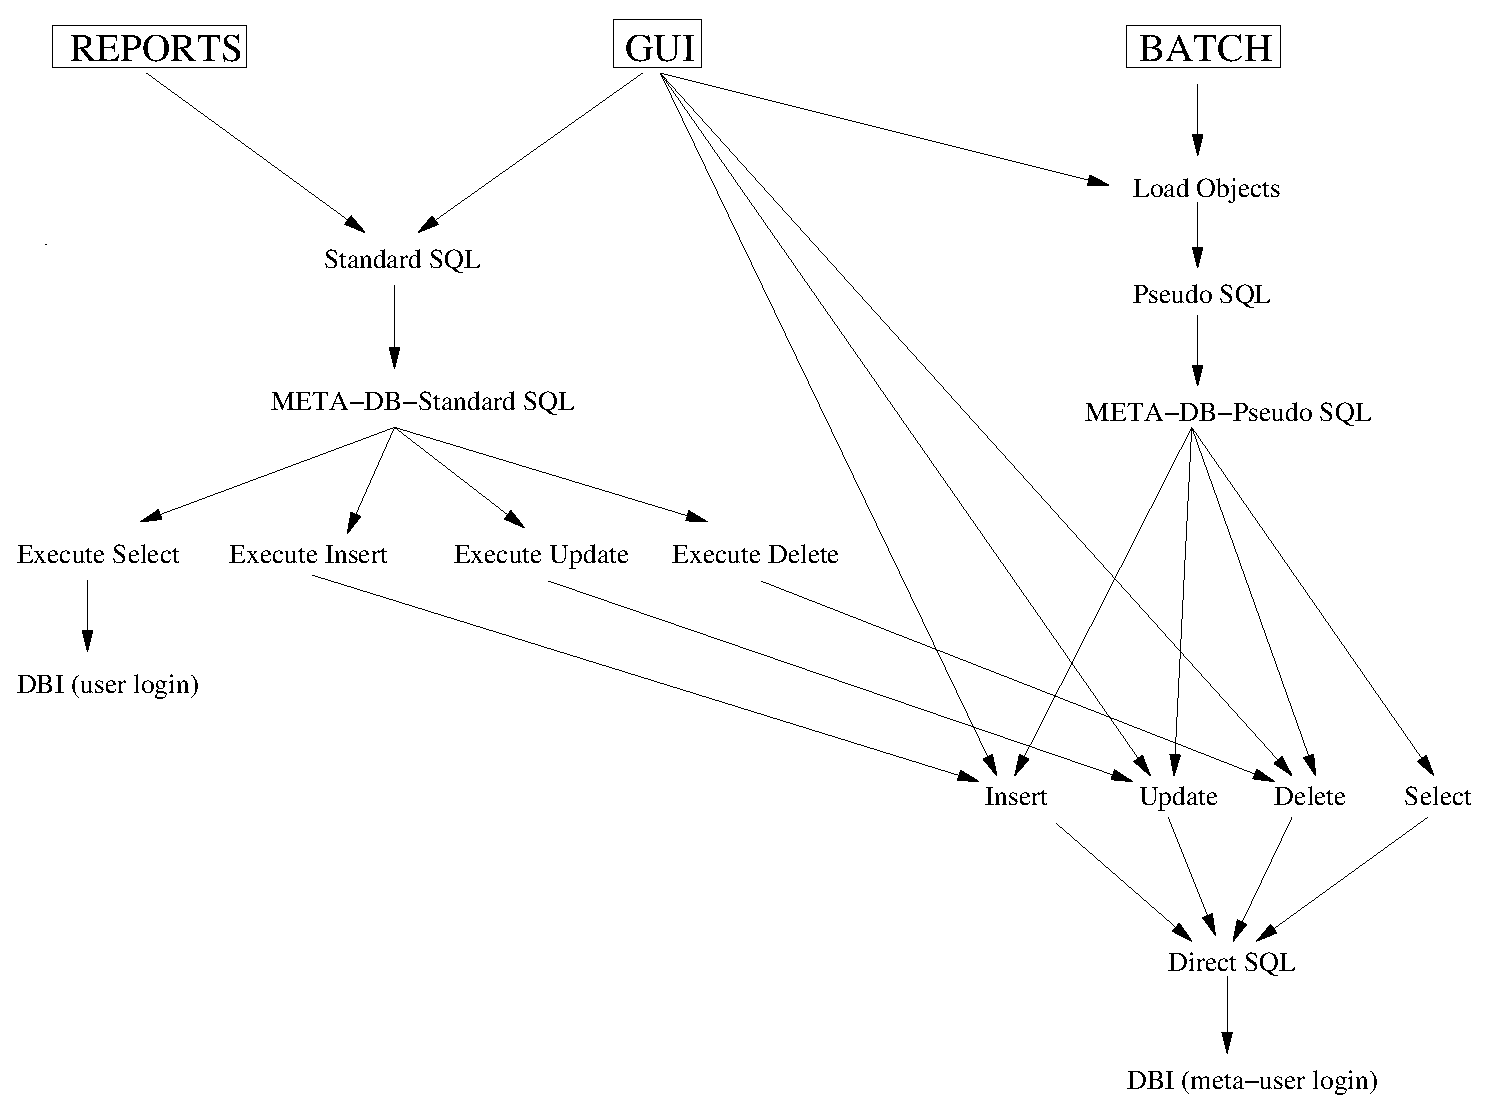
\includegraphics[scale=0.5]{./meta-layer/meta1.eps}
   \caption{}
\label{fig:meta1}
\end{figure}
\begin{figure}
   \centering
   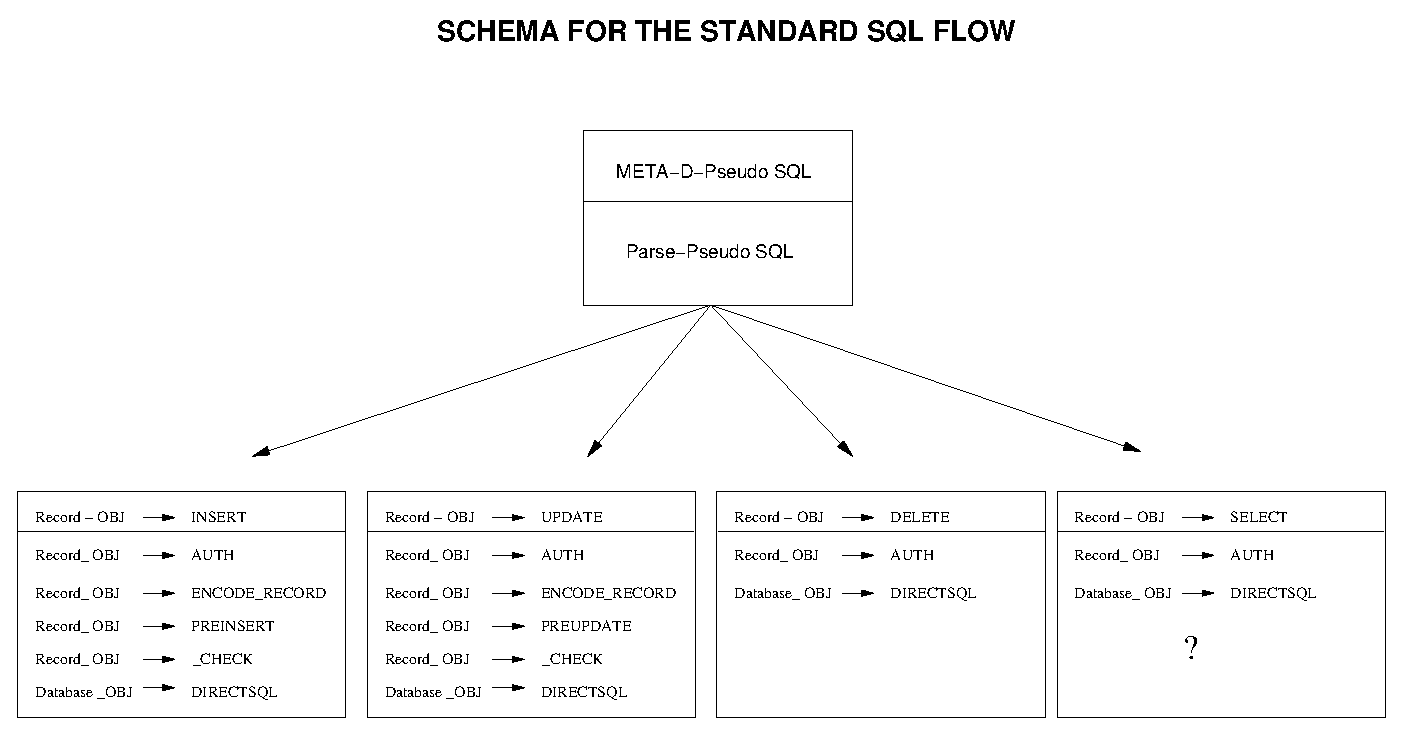
\includegraphics[scale=0.5]{./meta-layer/meta2.eps}
   \caption{}
   \label{fig:meta2}
\end{figure}

 
\section{PseudoSQL language definition}

In this chapter the formal definition of the PseudoSQL language is described.

The PseudoSQL has only INSERT, UPDATE, DELETE and SELECT \index{SELECT} statement.

\begin{verbatim}
 <pseudosql_statement> ::= <insert_statement> |
 			   <update_statement> |
			   <delete_statement> |
			   <select_statement> 
 \end{verbatim}


\subsection{INSERT}
\begin{verbatim}
    <insert_statement> ::= 'INSERT INTO  <table_name>
    				 ( <column_name> {, <column_name> })
                                  VALUES ( <value> {, <value> })'

	 <table_name> ::=>  <identifier> 

	 <identifier> ::= LETTER{LETTER|DIGIT}

	 <column_name> ::= <identifier> 

	 <value> ::= <scalar>|<string>|<variable>|<function> 

	 <scalar> ::= DIGIT{DIGIT}|DIGIT{DIGIT}.DIGIT{DIGIT}

	 <string> ::= ''{LETTER|DIGIT}''

	 <variable> ::= $<hash_key>[<external_fields>]

	 <hash_key> ::= <identifier> 

	 <external_fields> ::=[<field_list>]|[] 
	 here [] means square brackets, not optional element

	 <field_list> ::= ``<hash_key>{,<hash_key>}''

	 <function> ::= concat( <item> , <item> {,item})

	 <item> ::= <value>|<variable>|<string>.<variable>|<variable>.<string> 

\end{verbatim}

\subsection{UPDATE}

\begin{verbatim}


 <update_statement> ::= 'UPDATE  <table_name>
                         SET  <column_name> = <value> {, <column\_name> = <value> }
                         [WHERE  <where_clause> ]'

 <where_clause> ::= <column_name><operator><value>[ <AND|OR> <column_name><operator><value> ]

\end{verbatim}

\subsection{DELETE}

\begin{verbatim}

 <delete_statement> ::= 'DELETE FROM  <table_name>  [WHERE  <where_clause> ]'

\end{verbatim}

\subsection{SELECT}

\begin{verbatim}
 <select_statement> ::= 'SELECT  <variable> {, <variable> }
                         FROM  <table_name>
                         [WHERE  <where_clause> ]'

\end{verbatim}

\section{PseudoSQL flow}

\textbf{Subroutine name:} meta\_db\_PseudoSQL

\textbf{Input:} PseudoSQL - string

\textbf{Output:} 

\textbf{Description:}

\begin{enumerate}
\item Parses the PseudoSQL string using the Parse\_PseudoSQL subroutine
- to be written 
\item Executes the statement by call to a responding record object method:
{}``insert'', {}``update'' or {}``delete'';
\end{enumerate}
\textbf{Subroutine name:} Parse\_PseudoSQL

\textbf{Input:} PseudoSQL - string

\textbf{Output:} Record object filled with the data from the PseudoSQL
string

\textbf{Description: }

\begin{enumerate}
\item Parses the input string - gets the action name, table, column names,
column values and the where clause of the PseudoSQL - to be written 
\item Creates links between LO keys and database columns. These links will be used for targeting the errors, that may come from the underlying levels - to be written
\item Modifies and encodes the where clause and query the database for the
rowid of the first record responding to this where clause - to be
written
\item Creates record(table) object for the table parsed from the string:
my \$thisrecord = Apiis::DataBase::Record-> new( tablename =>  \$table,
); 
\item Fills the columns values from the PseudoSQL statement and the rowid
in the responding column objects using the record object method {}``extdata''
: \$record-> column(\$column\_name)-> extdata(\$column\_value); 
\end{enumerate}

\section{Standard SQL flow}

\textbf{Subroutine name:} meta\_db\_StandardSQL

\textbf{Input:} ordinary SQL - string

\textbf{Output:} 

\textbf{Description:}

\begin{enumerate}
\item Recognizes the sql action and if it is {}``SELECT'' executes it
through the view system using subroutine {}``ExecuteSelect'' 
\item In case of INSERT, UPDATE or DELETE parses the SQL string using the statement object from APIIS/DataBase/SQL/Statement.pm 
\item Calls the responding subroutine: {}``ExecuteInsert'', {}``ExecuteUpdate'' or {}``ExecuteDelete''

\end{enumerate}
\textbf{Subroutine name:} ExecuteSelect

\textbf{Input:} ordinary SQL SELECT statement- string

\textbf{Output:} Statement handle 

\textbf{Description:}

\begin{enumerate}
\item Connects to the database with the user login and executes the Select statement. For each user we will have also a database account and user's own schema(namespace) in the database. This schema will have the same name as the user database login and in this schema all original tables will be masked with views with the same names. For each table we will have a view that is a subset of the original table based on the access rights of the user. The user will have only read access to his schema and no access rights for the rest of the database   - to be written
\end{enumerate}

\textbf{Subroutine name:} ExecuteInsert

\textbf{Input:} parsed sql statement object

\textbf{Output:} 

\textbf{Description: }
\begin{enumerate}
\item Creates record(table) object for the table returned by the statement object; 
\item Fills the columns values from the statement in the responding column objects using the record object method {}``intdata''
\item Executes the statement by call to a responding record object method:
{}``insert'';

\end{enumerate}


\textbf{Subroutine name:} ExecuteUpdate

\textbf{Input:} parsed sql statement object

\textbf{Output:} 

\textbf{Description: }

\begin{enumerate}
\item Creates record(table) object for the table returned by the statement object; 
\item Fills the columns values from the statement in the responding column objects using the record object method {}``intdata''
\item Queries the database with the where clause returned from the statement object and gets the oids of all responding records;
\item Looping through the query results, fills the oid column in the record object with the value from the query and executes the statement by call to a responding record object method:{}``update'';

\end{enumerate}


\textbf{Subroutine name:} ExecuteDelete

\textbf{Input:} parsed sql statement object

\textbf{Output:} 

\textbf{Description: }
\begin{enumerate}
\item Creates record(table) object for the table returned by the statement object; 
\item Queries the database with the where clause returned from the statement object and gets the oids of all responding records;
\item Looping through the query results, fills the oid column in the record object with the value from the query and executes the statement by call to a responding record object method:{}``delete'';

\end{enumerate}


\section{Used record object methods}

\textbf{Method name:} insert 

\textbf{Input:} Record object filled with the data from the PseudoSQL
string 

\textbf{Output:} 

\textbf{Description:} 

\begin{enumerate}
\item Verifies if the user has appropriate rights to access the filled columns
in the record object using the record object method {}``auth''. Normally at this stage the record object should  contain only user data and the meta-fields are not set by the system yet;
\item If the record object is not encoded applies the modify rules from the model file to the external record data using record object method {}``\_modify''; 
\item If the record object is not encoded, encodes the external values to internal ones using the method {}``encode\_record''; 
\item Runs  all "PREINSERT" triggers - this is the place where the meta-fields like last\_change\_user are filled;
\item Checks the business rules using the record object method {}``\_check''. The checking is done always on the internal values; 
\item Creates ordinary SQL statement and executes it via {}``directsql'' method of the database object
\end{enumerate}

\textbf{Method name:} update 

\textbf{Input:} Record object filled with the data from the PseudoSQL
string 

\textbf{Output:} 

\textbf{Description:} 

\begin{enumerate}
\item Verifies if the user has appropriate rights to access the filled columns
in the record object using the record object method {}``auth''. Normally at this stage the record object should  contain only user data and the meta-fields are not set by the system yet;
\item If the record object is not encoded applies the modify rules from the model file to the external record data using record object method {}``\_modify''; 
\item If the record object is not encoded, encodes the external values to internal ones using the method {}``encode\_record''; 
\item Runs  all "PREUPDATE" triggers - this is the place where the meta-fields like last\_change\_user are filled;
\item Checks the business rules using the record object method {}``\_check''. The checking is done always on the internal values; 
\item Creates ordinary SQL statement and executes it via {}``directsql'' method of the database object
\end{enumerate}

\textbf{Method name:} delete 

\textbf{Input:} Record object filled with the data from the PseudoSQL string

\textbf{Output: }

\textbf{Description:} 

\begin{enumerate}
\item Verifies if the user has appropriate rights to access the filled columns
in the record object using the record object method {}``auth''. Normally at this stage the record object should  contain only user data and the meta-fields are not set by the system yet;
\item Runs  all "PREDELETE" triggers - in case of delete there are not any meta-fields to be filled, but maybe we will need this trigger for another purpose - referential integrity check;
\item Creates ordinary SQL statement and executes it via {}``directsql'' method of the database object
\end{enumerate}


\textbf{Method name:} auth 

\textbf{Input:} Record object filled with the data from the PseudoSQL
string 

\textbf{Output:} Additional where clause for the sql statement - string 

\textbf{Description:} 

\begin{enumerate}
\item Reads from the database the user access rights for this table and
action 
\item Verifies if the user has appropriate access to these columns 
\item Generates additional where clause to filter the owner
\end{enumerate}

